\documentclass{standalone}
\usepackage{tikz}
\usetikzlibrary{patterns, positioning}
\usepackage[sfdefault]{ClearSans} %% option 'sfdefault' activates Clear Sans as the default text font
\usepackage[T1]{fontenc}

\begin{document}
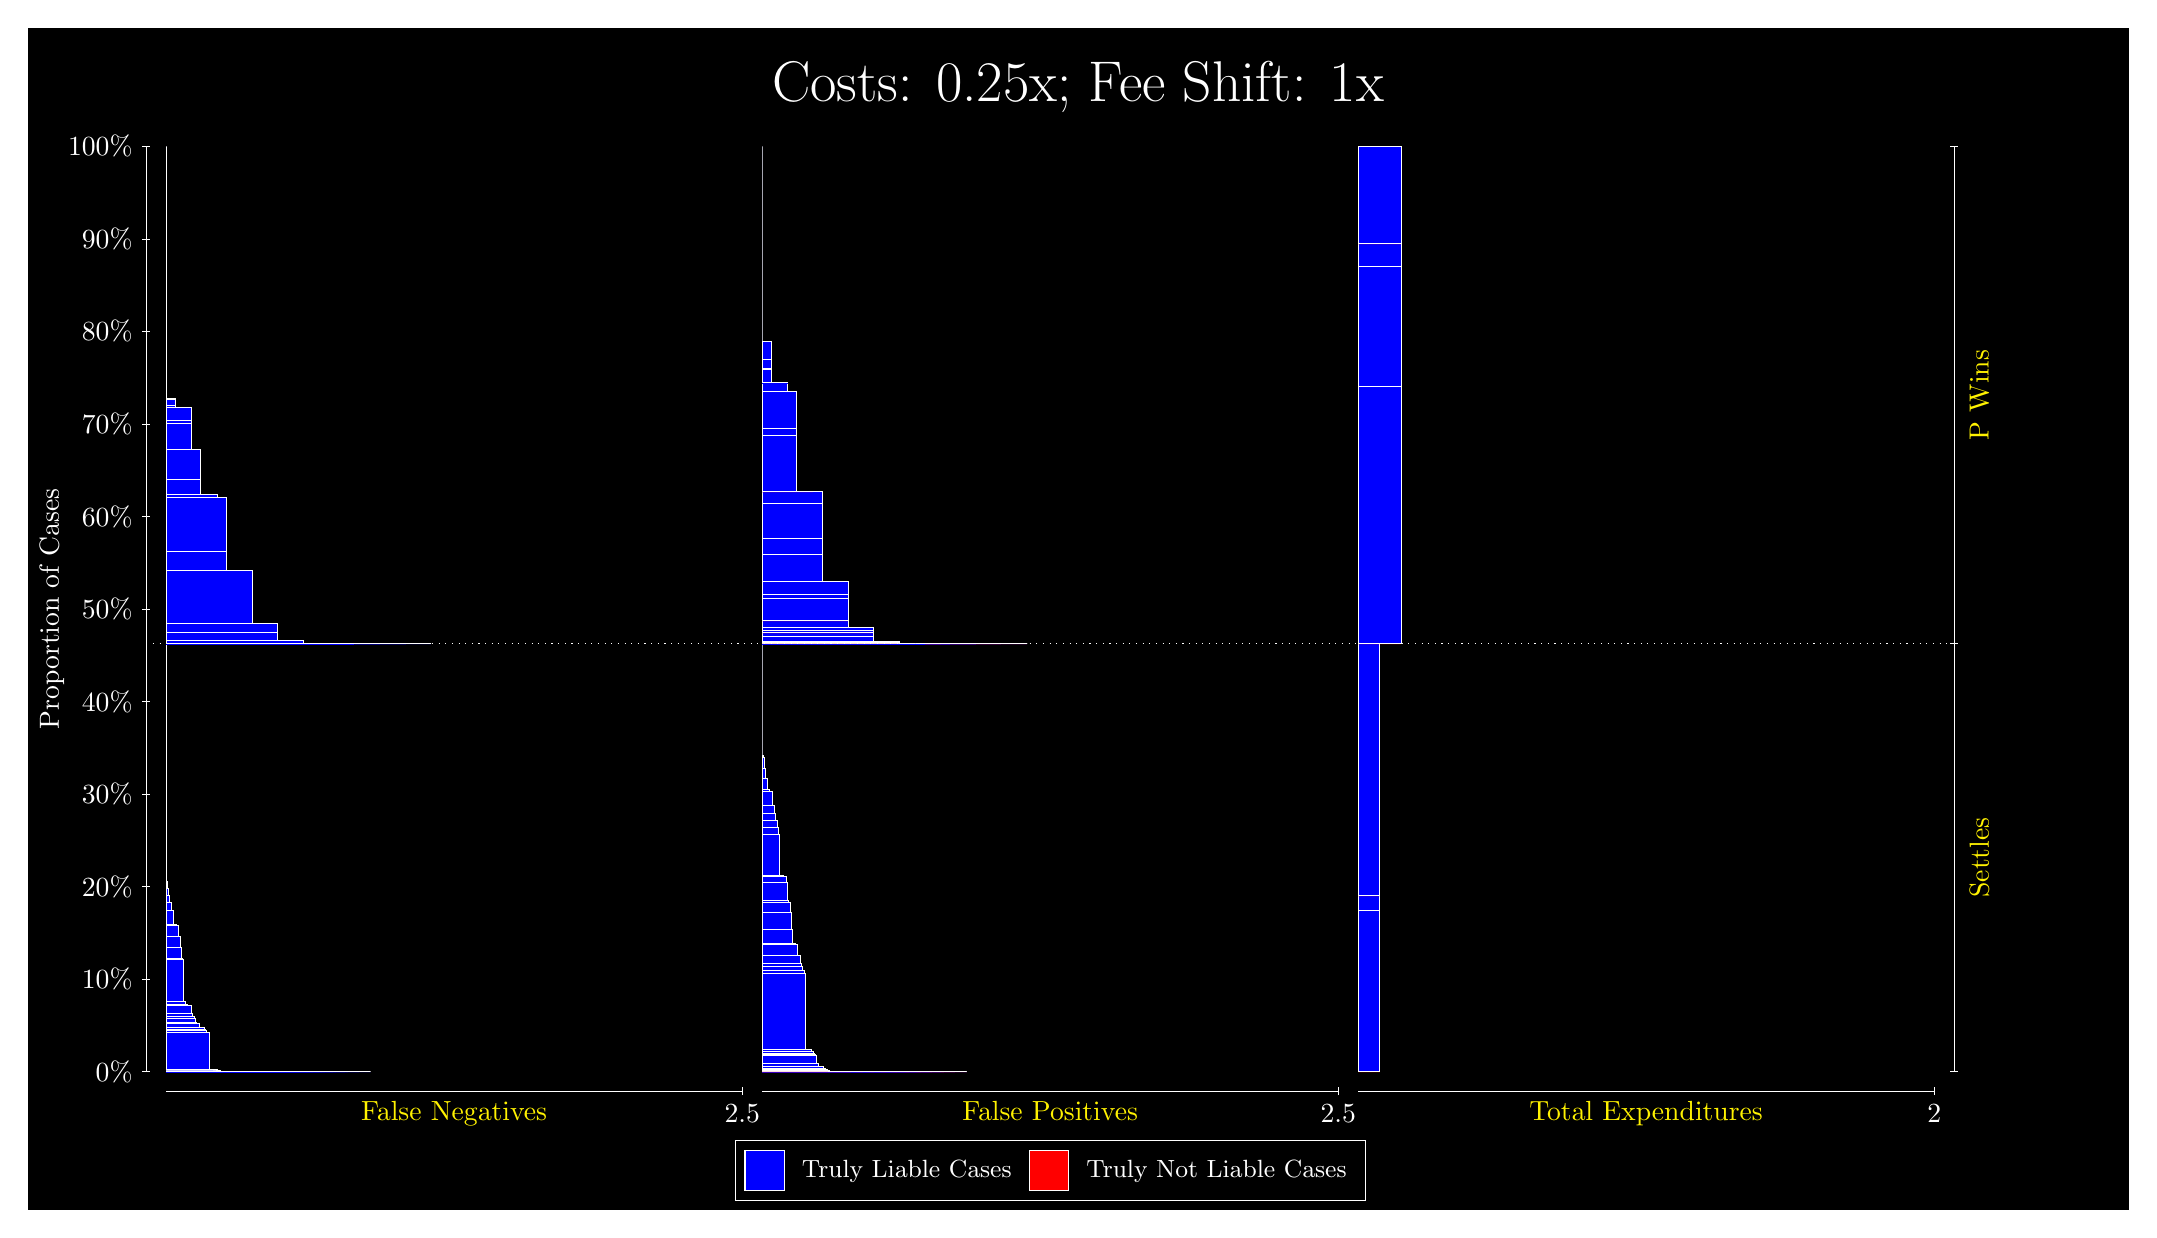
\begin{tikzpicture}
\draw[fill=black] (0,0) rectangle (26.667,15);
\draw[text=white] (0,13.5) rectangle (26.667,15) node[midway] {\huge Costs: 0.25x; Fee Shift: 1x};
\draw[white, very thin] (1.5,1.75) -- (1.5,13.5);
\node[rotate=90, text=white, anchor=center] at (0.3, 7.625) {Proportion of Cases};
\draw[white, very thin] (1.45,1.75) -- (1.55,1.75);
\node[text=white, anchor=east] at (1.45, 1.75) {0\%};
\draw[white, very thin] (1.45,2.925) -- (1.55,2.925);
\node[text=white, anchor=east] at (1.45, 2.925) {10\%};
\draw[white, very thin] (1.45,4.1) -- (1.55,4.1);
\node[text=white, anchor=east] at (1.45, 4.1) {20\%};
\draw[white, very thin] (1.45,5.275) -- (1.55,5.275);
\node[text=white, anchor=east] at (1.45, 5.275) {30\%};
\draw[white, very thin] (1.45,6.45) -- (1.55,6.45);
\node[text=white, anchor=east] at (1.45, 6.45) {40\%};
\draw[white, very thin] (1.45,7.625) -- (1.55,7.625);
\node[text=white, anchor=east] at (1.45, 7.625) {50\%};
\draw[white, very thin] (1.45,8.8) -- (1.55,8.8);
\node[text=white, anchor=east] at (1.45, 8.8) {60\%};
\draw[white, very thin] (1.45,9.975) -- (1.55,9.975);
\node[text=white, anchor=east] at (1.45, 9.975) {70\%};
\draw[white, very thin] (1.45,11.15) -- (1.55,11.15);
\node[text=white, anchor=east] at (1.45, 11.15) {80\%};
\draw[white, very thin] (1.45,12.325) -- (1.55,12.325);
\node[text=white, anchor=east] at (1.45, 12.325) {90\%};
\draw[white, very thin] (1.45,13.5) -- (1.55,13.5);
\node[text=white, anchor=east] at (1.45, 13.5) {100\%};

\draw[white, very thin] (24.457,1.75) -- (24.457,13.5);
\draw[white, very thin] (24.407,1.75) -- (24.507,1.75);
\node[anchor=west] at (24.407, 1.75) {};
\draw[white, very thin] (24.407,7.184) -- (24.507,7.184);
\node[anchor=west] at (24.407, 7.184) {};
\draw[white, very thin] (24.407,13.5) -- (24.507,13.5);
\node[anchor=west] at (24.407, 13.5) {};

\draw[white, very thin, fill=blue] (1.75,1.75) rectangle (4.3482,1.75);
\draw[white, very thin, fill=blue] (1.75,1.75) rectangle (4.2018,1.75);
\draw[white, very thin, fill=blue] (1.75,1.75) rectangle (4.0554,1.75);
\draw[white, very thin, fill=blue] (1.75,1.75) rectangle (4.0229,1.75);
\draw[white, very thin, fill=blue] (1.75,1.75) rectangle (3.9091,1.75);
\draw[white, very thin, fill=blue] (1.75,1.75) rectangle (3.8765,1.75);
\draw[white, very thin, fill=blue] (1.75,1.75) rectangle (3.7627,1.75);
\draw[white, very thin, fill=blue] (1.75,1.75) rectangle (3.7302,1.75);
\draw[white, very thin, fill=blue] (1.75,1.75) rectangle (3.6976,1.75);
\draw[white, very thin, fill=blue] (1.75,1.75) rectangle (3.6163,1.75);
\draw[white, very thin, fill=blue] (1.75,1.75) rectangle (3.5838,1.75);
\draw[white, very thin, fill=blue] (1.75,1.75) rectangle (3.5513,1.75);
\draw[white, very thin, fill=blue] (1.75,1.75) rectangle (3.4699,1.75);
\draw[white, very thin, fill=blue] (1.75,1.75) rectangle (3.4374,1.75);
\draw[white, very thin, fill=blue] (1.75,1.75) rectangle (3.4049,1.75);
\draw[white, very thin, fill=blue] (1.75,1.75) rectangle (3.3723,1.75);
\draw[white, very thin, fill=blue] (1.75,1.75) rectangle (3.3236,1.75);
\draw[white, very thin, fill=blue] (1.75,1.75) rectangle (3.291,1.75);
\draw[white, very thin, fill=blue] (1.75,1.75) rectangle (3.2585,1.75);
\draw[white, very thin, fill=blue] (1.75,1.75) rectangle (3.226,1.75);
\draw[white, very thin, fill=blue] (1.75,1.75) rectangle (3.1772,1.75);
\draw[white, very thin, fill=blue] (1.75,1.75) rectangle (3.1447,1.75);
\draw[white, very thin, fill=blue] (1.75,1.75) rectangle (3.1121,1.75);
\draw[white, very thin, fill=blue] (1.75,1.75) rectangle (3.0796,1.75);
\draw[white, very thin, fill=blue] (1.75,1.75) rectangle (3.0471,1.75);
\draw[white, very thin, fill=blue] (1.75,1.75) rectangle (3.0308,1.75);
\draw[white, very thin, fill=blue] (1.75,1.75) rectangle (2.9983,1.75);
\draw[white, very thin, fill=blue] (1.75,1.75) rectangle (2.9657,1.75);
\draw[white, very thin, fill=blue] (1.75,1.75) rectangle (2.9332,1.75);
\draw[white, very thin, fill=blue] (1.75,1.75) rectangle (2.9007,1.75);
\draw[white, very thin, fill=blue] (1.75,1.75) rectangle (2.8844,1.75);
\draw[white, very thin, fill=blue] (1.75,1.75) rectangle (2.8519,1.75);
\draw[white, very thin, fill=blue] (1.75,1.75) rectangle (2.8194,1.75);
\draw[white, very thin, fill=blue] (1.75,1.75) rectangle (2.7868,1.75);
\draw[white, very thin, fill=blue] (1.75,1.75) rectangle (2.7543,1.75);
\draw[white, very thin, fill=blue] (1.75,1.75) rectangle (2.738,1.7501);
\draw[white, very thin, fill=blue] (1.75,1.7501) rectangle (2.7218,1.7501);
\draw[white, very thin, fill=blue] (1.75,1.7501) rectangle (2.7055,1.7501);
\draw[white, very thin, fill=blue] (1.75,1.7501) rectangle (2.673,1.7501);
\draw[white, very thin, fill=blue] (1.75,1.7501) rectangle (2.6405,1.7502);
\draw[white, very thin, fill=blue] (1.75,1.7502) rectangle (2.6079,1.7504);
\draw[white, very thin, fill=blue] (1.75,1.7504) rectangle (2.5917,1.7516);
\draw[white, very thin, fill=blue] (1.75,1.7516) rectangle (2.5754,1.7521);
\draw[white, very thin, fill=blue] (1.75,1.7521) rectangle (2.5591,1.7526);
\draw[white, very thin, fill=blue] (1.75,1.7526) rectangle (2.5266,1.7526);
\draw[white, very thin, fill=blue] (1.75,1.7526) rectangle (2.4941,1.7548);
\draw[white, very thin, fill=blue] (1.75,1.7548) rectangle (2.4616,1.7552);
\draw[white, very thin, fill=blue] (1.75,1.7552) rectangle (2.4453,1.7644);
\draw[white, very thin, fill=blue] (1.75,1.7644) rectangle (2.429,1.7661);
\draw[white, very thin, fill=blue] (1.75,1.7661) rectangle (2.4128,1.7682);
\draw[white, very thin, fill=blue] (1.75,1.7682) rectangle (2.3965,1.7734);
\draw[white, very thin, fill=blue] (1.75,1.7734) rectangle (2.3802,1.7735);
\draw[white, very thin, fill=blue] (1.75,1.7735) rectangle (2.3477,1.7736);
\draw[white, very thin, fill=blue] (1.75,1.7736) rectangle (2.3152,1.778);
\draw[white, very thin, fill=blue] (1.75,1.778) rectangle (2.2989,2.2422);
\draw[white, very thin, fill=blue] (1.75,2.2422) rectangle (2.2827,2.2467);
\draw[white, very thin, fill=blue] (1.75,2.2467) rectangle (2.2664,2.2717);
\draw[white, very thin, fill=blue] (1.75,2.2717) rectangle (2.2501,2.2906);
\draw[white, very thin, fill=blue] (1.75,2.2906) rectangle (2.2339,2.3099);
\draw[white, very thin, fill=blue] (1.75,2.3099) rectangle (2.2013,2.3126);
\draw[white, very thin, fill=blue] (1.75,2.3126) rectangle (2.1688,2.3571);
\draw[white, very thin, fill=blue] (1.75,2.3571) rectangle (2.1363,2.3743);
\draw[white, very thin, fill=blue] (1.75,2.3743) rectangle (2.12,2.4254);
\draw[white, very thin, fill=blue] (1.75,2.4254) rectangle (2.1037,2.4554);
\draw[white, very thin, fill=blue] (1.75,2.4554) rectangle (2.0875,2.4857);
\draw[white, very thin, fill=blue] (1.75,2.4857) rectangle (2.0712,2.5944);
\draw[white, very thin, fill=blue] (1.75,2.5944) rectangle (2.055,2.5962);
\draw[white, very thin, fill=blue] (1.75,2.5962) rectangle (2.0224,2.5979);
\draw[white, very thin, fill=blue] (1.75,2.5979) rectangle (1.9899,2.6428);
\draw[white, very thin, fill=blue] (1.75,2.6428) rectangle (1.9736,3.1693);
\draw[white, very thin, fill=blue] (1.75,3.1693) rectangle (1.9574,3.1929);
\draw[white, very thin, fill=blue] (1.75,3.1929) rectangle (1.9411,3.327);
\draw[white, very thin, fill=blue] (1.75,3.327) rectangle (1.9248,3.4647);
\draw[white, very thin, fill=blue] (1.75,3.4647) rectangle (1.9086,3.6013);
\draw[white, very thin, fill=blue] (1.75,3.6013) rectangle (1.876,3.6189);
\draw[white, very thin, fill=blue] (1.75,3.6189) rectangle (1.8435,3.7964);
\draw[white, very thin, fill=blue] (1.75,3.7964) rectangle (1.811,3.9052);
\draw[white, very thin, fill=blue] (1.75,3.9052) rectangle (1.7947,3.9922);
\draw[white, very thin, fill=blue] (1.75,3.9922) rectangle (1.7785,4.0791);
\draw[white, very thin, fill=blue] (1.75,4.0791) rectangle (1.7622,4.165);
\draw[white, very thin, fill=red] (1.75,4.165) rectangle (1.75,4.165);
\draw[white, very thin, fill=blue] (1.75,4.165) rectangle (1.75,7.184);
\draw[white, very thin, fill=blue] (1.75,7.184) rectangle (5.1167,7.184);
\draw[white, very thin, fill=blue] (1.75,7.184) rectangle (4.7914,7.184);
\draw[white, very thin, fill=blue] (1.75,7.184) rectangle (4.7914,7.184);
\draw[white, very thin, fill=blue] (1.75,7.184) rectangle (4.4661,7.184);
\draw[white, very thin, fill=blue] (1.75,7.184) rectangle (4.4661,7.184);
\draw[white, very thin, fill=blue] (1.75,7.184) rectangle (4.1408,7.1844);
\draw[white, very thin, fill=blue] (1.75,7.1844) rectangle (4.027,7.1844);
\draw[white, very thin, fill=blue] (1.75,7.1844) rectangle (3.8155,7.1877);
\draw[white, very thin, fill=blue] (1.75,7.1877) rectangle (3.8155,7.1895);
\draw[white, very thin, fill=blue] (1.75,7.1895) rectangle (3.7017,7.1895);
\draw[white, very thin, fill=blue] (1.75,7.1895) rectangle (3.7017,7.1895);
\draw[white, very thin, fill=blue] (1.75,7.1895) rectangle (3.4903,7.2316);
\draw[white, very thin, fill=blue] (1.75,7.2316) rectangle (3.3764,7.2316);
\draw[white, very thin, fill=blue] (1.75,7.2316) rectangle (3.165,7.3328);
\draw[white, very thin, fill=blue] (1.75,7.3328) rectangle (3.165,7.4489);
\draw[white, very thin, fill=blue] (1.75,7.4489) rectangle (3.0511,7.4489);
\draw[white, very thin, fill=blue] (1.75,7.4489) rectangle (3.0511,7.4489);
\draw[white, very thin, fill=blue] (1.75,7.4489) rectangle (2.8397,8.1204);
\draw[white, very thin, fill=blue] (1.75,8.1204) rectangle (2.7258,8.1211);
\draw[white, very thin, fill=blue] (1.75,8.1211) rectangle (2.7258,8.1211);
\draw[white, very thin, fill=blue] (1.75,8.1211) rectangle (2.7258,8.1215);
\draw[white, very thin, fill=blue] (1.75,8.1215) rectangle (2.5144,8.3595);
\draw[white, very thin, fill=blue] (1.75,8.3595) rectangle (2.5144,9.043);
\draw[white, very thin, fill=blue] (1.75,9.043) rectangle (2.4006,9.0438);
\draw[white, very thin, fill=blue] (1.75,9.0438) rectangle (2.4006,9.0855);
\draw[white, very thin, fill=blue] (1.75,9.0855) rectangle (2.1891,9.2728);
\draw[white, very thin, fill=blue] (1.75,9.2728) rectangle (2.1891,9.6563);
\draw[white, very thin, fill=blue] (1.75,9.6563) rectangle (2.0753,9.9834);
\draw[white, very thin, fill=blue] (1.75,9.9834) rectangle (2.0753,10.015);
\draw[white, very thin, fill=blue] (1.75,10.015) rectangle (2.0753,10.184);
\draw[white, very thin, fill=blue] (1.75,10.184) rectangle (1.8638,10.185);
\draw[white, very thin, fill=blue] (1.75,10.185) rectangle (1.8638,10.208);
\draw[white, very thin, fill=blue] (1.75,10.208) rectangle (1.8638,10.293);
\draw[white, very thin, fill=blue] (1.75,10.293) rectangle (1.8638,10.294);
\draw[white, very thin, fill=red] (1.75,10.294) rectangle (1.75,10.294);
\draw[white, very thin, fill=blue] (1.75,10.294) rectangle (1.75,13.5);
\draw[white, very thin, fill=red] (9.3189,1.75) rectangle (11.917,1.75);
\draw[white, very thin, fill=blue] (9.3189,1.75) rectangle (11.917,1.75);
\draw[white, very thin, fill=red] (9.3189,1.75) rectangle (11.771,1.75);
\draw[white, very thin, fill=blue] (9.3189,1.75) rectangle (11.771,1.75);
\draw[white, very thin, fill=red] (9.3189,1.75) rectangle (11.624,1.75);
\draw[white, very thin, fill=blue] (9.3189,1.75) rectangle (11.624,1.75);
\draw[white, very thin, fill=blue] (9.3189,1.75) rectangle (11.592,1.75);
\draw[white, very thin, fill=red] (9.3189,1.75) rectangle (11.478,1.75);
\draw[white, very thin, fill=blue] (9.3189,1.75) rectangle (11.478,1.75);
\draw[white, very thin, fill=blue] (9.3189,1.75) rectangle (11.445,1.75);
\draw[white, very thin, fill=red] (9.3189,1.75) rectangle (11.332,1.75);
\draw[white, very thin, fill=blue] (9.3189,1.75) rectangle (11.332,1.75);
\draw[white, very thin, fill=blue] (9.3189,1.75) rectangle (11.299,1.75);
\draw[white, very thin, fill=blue] (9.3189,1.75) rectangle (11.266,1.75);
\draw[white, very thin, fill=red] (9.3189,1.75) rectangle (11.185,1.75);
\draw[white, very thin, fill=blue] (9.3189,1.75) rectangle (11.185,1.75);
\draw[white, very thin, fill=blue] (9.3189,1.75) rectangle (11.153,1.75);
\draw[white, very thin, fill=blue] (9.3189,1.75) rectangle (11.12,1.75);
\draw[white, very thin, fill=red] (9.3189,1.75) rectangle (11.039,1.75);
\draw[white, very thin, fill=blue] (9.3189,1.75) rectangle (11.039,1.75);
\draw[white, very thin, fill=blue] (9.3189,1.75) rectangle (11.006,1.75);
\draw[white, very thin, fill=blue] (9.3189,1.75) rectangle (10.974,1.75);
\draw[white, very thin, fill=blue] (9.3189,1.75) rectangle (10.941,1.75);
\draw[white, very thin, fill=red] (9.3189,1.75) rectangle (10.892,1.75);
\draw[white, very thin, fill=blue] (9.3189,1.75) rectangle (10.892,1.75);
\draw[white, very thin, fill=blue] (9.3189,1.75) rectangle (10.86,1.75);
\draw[white, very thin, fill=blue] (9.3189,1.75) rectangle (10.827,1.75);
\draw[white, very thin, fill=blue] (9.3189,1.75) rectangle (10.795,1.75);
\draw[white, very thin, fill=red] (9.3189,1.75) rectangle (10.746,1.75);
\draw[white, very thin, fill=blue] (9.3189,1.75) rectangle (10.746,1.75);
\draw[white, very thin, fill=blue] (9.3189,1.75) rectangle (10.714,1.75);
\draw[white, very thin, fill=blue] (9.3189,1.75) rectangle (10.681,1.75);
\draw[white, very thin, fill=blue] (9.3189,1.75) rectangle (10.648,1.75);
\draw[white, very thin, fill=blue] (9.3189,1.75) rectangle (10.616,1.75);
\draw[white, very thin, fill=red] (9.3189,1.75) rectangle (10.6,1.75);
\draw[white, very thin, fill=blue] (9.3189,1.75) rectangle (10.6,1.7501);
\draw[white, very thin, fill=blue] (9.3189,1.7501) rectangle (10.567,1.7501);
\draw[white, very thin, fill=blue] (9.3189,1.7501) rectangle (10.535,1.7501);
\draw[white, very thin, fill=blue] (9.3189,1.7501) rectangle (10.502,1.7501);
\draw[white, very thin, fill=blue] (9.3189,1.7501) rectangle (10.47,1.7502);
\draw[white, very thin, fill=red] (9.3189,1.7502) rectangle (10.453,1.7502);
\draw[white, very thin, fill=blue] (9.3189,1.7502) rectangle (10.453,1.7511);
\draw[white, very thin, fill=blue] (9.3189,1.7511) rectangle (10.421,1.7516);
\draw[white, very thin, fill=blue] (9.3189,1.7516) rectangle (10.388,1.7516);
\draw[white, very thin, fill=blue] (9.3189,1.7516) rectangle (10.356,1.7538);
\draw[white, very thin, fill=blue] (9.3189,1.7538) rectangle (10.323,1.7543);
\draw[white, very thin, fill=red] (9.3189,1.7543) rectangle (10.307,1.7543);
\draw[white, very thin, fill=blue] (9.3189,1.7543) rectangle (10.307,1.7547);
\draw[white, very thin, fill=blue] (9.3189,1.7547) rectangle (10.291,1.7552);
\draw[white, very thin, fill=blue] (9.3189,1.7552) rectangle (10.274,1.7572);
\draw[white, very thin, fill=blue] (9.3189,1.7572) rectangle (10.242,1.7573);
\draw[white, very thin, fill=blue] (9.3189,1.7573) rectangle (10.209,1.7574);
\draw[white, very thin, fill=blue] (9.3189,1.7574) rectangle (10.177,1.7618);
\draw[white, very thin, fill=red] (9.3189,1.7618) rectangle (10.161,1.7618);
\draw[white, very thin, fill=blue] (9.3189,1.7618) rectangle (10.161,1.771);
\draw[white, very thin, fill=blue] (9.3189,1.771) rectangle (10.144,1.7728);
\draw[white, very thin, fill=blue] (9.3189,1.7728) rectangle (10.128,1.7925);
\draw[white, very thin, fill=blue] (9.3189,1.7925) rectangle (10.095,1.8117);
\draw[white, very thin, fill=blue] (9.3189,1.8117) rectangle (10.063,1.8144);
\draw[white, very thin, fill=blue] (9.3189,1.8144) rectangle (10.03,1.859);
\draw[white, very thin, fill=red] (9.3189,1.859) rectangle (10.014,1.859);
\draw[white, very thin, fill=blue] (9.3189,1.859) rectangle (10.014,1.952);
\draw[white, very thin, fill=blue] (9.3189,1.952) rectangle (9.9979,1.9738);
\draw[white, very thin, fill=blue] (9.3189,1.9738) rectangle (9.9816,1.979);
\draw[white, very thin, fill=blue] (9.3189,1.979) rectangle (9.9654,2.0026);
\draw[white, very thin, fill=blue] (9.3189,2.0026) rectangle (9.9491,2.0331);
\draw[white, very thin, fill=blue] (9.3189,2.0331) rectangle (9.9166,2.0348);
\draw[white, very thin, fill=blue] (9.3189,2.0348) rectangle (9.884,2.0365);
\draw[white, very thin, fill=red] (9.3189,2.0365) rectangle (9.8678,2.0365);
\draw[white, very thin, fill=blue] (9.3189,2.0365) rectangle (9.8678,2.9954);
\draw[white, very thin, fill=blue] (9.3189,2.9954) rectangle (9.8515,3.0399);
\draw[white, very thin, fill=blue] (9.3189,3.0399) rectangle (9.8353,3.0909);
\draw[white, very thin, fill=blue] (9.3189,3.0909) rectangle (9.819,3.1209);
\draw[white, very thin, fill=blue] (9.3189,3.1209) rectangle (9.8027,3.231);
\draw[white, very thin, fill=blue] (9.3189,3.231) rectangle (9.7702,3.3671);
\draw[white, very thin, fill=blue] (9.3189,3.3671) rectangle (9.7377,3.3848);
\draw[white, very thin, fill=blue] (9.3189,3.3848) rectangle (9.7051,3.5626);
\draw[white, very thin, fill=blue] (9.3189,3.5626) rectangle (9.6889,3.7664);
\draw[white, very thin, fill=blue] (9.3189,3.7664) rectangle (9.6726,3.8988);
\draw[white, very thin, fill=blue] (9.3189,3.8988) rectangle (9.6563,3.9228);
\draw[white, very thin, fill=blue] (9.3189,3.9228) rectangle (9.6401,4.1475);
\draw[white, very thin, fill=blue] (9.3189,4.1475) rectangle (9.6238,4.2338);
\draw[white, very thin, fill=blue] (9.3189,4.2338) rectangle (9.5913,4.2382);
\draw[white, very thin, fill=blue] (9.3189,4.2382) rectangle (9.5588,4.2425);
\draw[white, very thin, fill=blue] (9.3189,4.2425) rectangle (9.5425,4.769);
\draw[white, very thin, fill=blue] (9.3189,4.769) rectangle (9.5262,4.8549);
\draw[white, very thin, fill=blue] (9.3189,4.8549) rectangle (9.51,4.9419);
\draw[white, very thin, fill=blue] (9.3189,4.9419) rectangle (9.4937,5.0288);
\draw[white, very thin, fill=blue] (9.3189,5.0288) rectangle (9.4774,5.1376);
\draw[white, very thin, fill=blue] (9.3189,5.1376) rectangle (9.4449,5.3151);
\draw[white, very thin, fill=blue] (9.3189,5.3151) rectangle (9.4124,5.3327);
\draw[white, very thin, fill=blue] (9.3189,5.3327) rectangle (9.3799,5.4693);
\draw[white, very thin, fill=blue] (9.3189,5.4693) rectangle (9.3636,5.607);
\draw[white, very thin, fill=blue] (9.3189,5.607) rectangle (9.3473,5.7411);
\draw[white, very thin, fill=blue] (9.3189,5.7411) rectangle (9.3311,5.7647);
\draw[white, very thin, fill=blue] (9.3189,5.7647) rectangle (9.3189,7.184);
\draw[white, very thin, fill=red] (9.3189,7.184) rectangle (12.686,7.184);
\draw[white, very thin, fill=blue] (9.3189,7.184) rectangle (12.686,7.184);
\draw[white, very thin, fill=red] (9.3189,7.184) rectangle (12.36,7.184);
\draw[white, very thin, fill=blue] (9.3189,7.184) rectangle (12.36,7.184);
\draw[white, very thin, fill=red] (9.3189,7.184) rectangle (12.035,7.184);
\draw[white, very thin, fill=blue] (9.3189,7.184) rectangle (12.035,7.184);
\draw[white, very thin, fill=blue] (9.3189,7.184) rectangle (12.035,7.184);
\draw[white, very thin, fill=blue] (9.3189,7.184) rectangle (12.035,7.184);
\draw[white, very thin, fill=red] (9.3189,7.184) rectangle (11.71,7.184);
\draw[white, very thin, fill=blue] (9.3189,7.184) rectangle (11.71,7.1842);
\draw[white, very thin, fill=blue] (9.3189,7.1842) rectangle (11.71,7.1843);
\draw[white, very thin, fill=red] (9.3189,7.1843) rectangle (11.596,7.1843);
\draw[white, very thin, fill=blue] (9.3189,7.1843) rectangle (11.596,7.1843);
\draw[white, very thin, fill=red] (9.3189,7.1843) rectangle (11.384,7.1843);
\draw[white, very thin, fill=blue] (9.3189,7.1843) rectangle (11.384,7.1853);
\draw[white, very thin, fill=blue] (9.3189,7.1853) rectangle (11.384,7.1879);
\draw[white, very thin, fill=blue] (9.3189,7.1879) rectangle (11.271,7.1879);
\draw[white, very thin, fill=red] (9.3189,7.1879) rectangle (11.271,7.1879);
\draw[white, very thin, fill=blue] (9.3189,7.1879) rectangle (11.271,7.1879);
\draw[white, very thin, fill=blue] (9.3189,7.1879) rectangle (11.059,7.198);
\draw[white, very thin, fill=red] (9.3189,7.198) rectangle (11.059,7.198);
\draw[white, very thin, fill=blue] (9.3189,7.198) rectangle (11.059,7.2054);
\draw[white, very thin, fill=blue] (9.3189,7.2054) rectangle (11.059,7.2199);
\draw[white, very thin, fill=red] (9.3189,7.2199) rectangle (10.945,7.2199);
\draw[white, very thin, fill=blue] (9.3189,7.2199) rectangle (10.945,7.2199);
\draw[white, very thin, fill=blue] (9.3189,7.2199) rectangle (10.734,7.2787);
\draw[white, very thin, fill=blue] (9.3189,7.2787) rectangle (10.734,7.3243);
\draw[white, very thin, fill=red] (9.3189,7.3243) rectangle (10.734,7.3243);
\draw[white, very thin, fill=blue] (9.3189,7.3243) rectangle (10.734,7.3602);
\draw[white, very thin, fill=blue] (9.3189,7.3602) rectangle (10.734,7.3927);
\draw[white, very thin, fill=blue] (9.3189,7.3927) rectangle (10.62,7.3927);
\draw[white, very thin, fill=red] (9.3189,7.3927) rectangle (10.62,7.3927);
\draw[white, very thin, fill=blue] (9.3189,7.3927) rectangle (10.62,7.3927);
\draw[white, very thin, fill=blue] (9.3189,7.3927) rectangle (10.409,7.4777);
\draw[white, very thin, fill=red] (9.3189,7.4777) rectangle (10.409,7.4777);
\draw[white, very thin, fill=blue] (9.3189,7.4777) rectangle (10.409,7.7617);
\draw[white, very thin, fill=blue] (9.3189,7.7617) rectangle (10.409,7.8092);
\draw[white, very thin, fill=blue] (9.3189,7.8092) rectangle (10.409,7.9734);
\draw[white, very thin, fill=blue] (9.3189,7.9734) rectangle (10.295,7.9734);
\draw[white, very thin, fill=red] (9.3189,7.9734) rectangle (10.295,7.9734);
\draw[white, very thin, fill=blue] (9.3189,7.9734) rectangle (10.295,7.9734);
\draw[white, very thin, fill=blue] (9.3189,7.9734) rectangle (10.083,8.3145);
\draw[white, very thin, fill=blue] (9.3189,8.3145) rectangle (10.083,8.5179);
\draw[white, very thin, fill=blue] (9.3189,8.5179) rectangle (10.083,8.9651);
\draw[white, very thin, fill=blue] (9.3189,8.9651) rectangle (10.083,9.1155);
\draw[white, very thin, fill=blue] (9.3189,9.1155) rectangle (9.9694,9.1155);
\draw[white, very thin, fill=red] (9.3189,9.1155) rectangle (9.9694,9.1155);
\draw[white, very thin, fill=blue] (9.3189,9.1155) rectangle (9.9694,9.1186);
\draw[white, very thin, fill=blue] (9.3189,9.1186) rectangle (9.758,9.8335);
\draw[white, very thin, fill=blue] (9.3189,9.8335) rectangle (9.758,9.9227);
\draw[white, very thin, fill=blue] (9.3189,9.9227) rectangle (9.758,10.39);
\draw[white, very thin, fill=blue] (9.3189,10.39) rectangle (9.6442,10.391);
\draw[white, very thin, fill=red] (9.3189,10.391) rectangle (9.6442,10.391);
\draw[white, very thin, fill=blue] (9.3189,10.391) rectangle (9.6442,10.499);
\draw[white, very thin, fill=blue] (9.3189,10.499) rectangle (9.6442,10.5);
\draw[white, very thin, fill=blue] (9.3189,10.5) rectangle (9.4327,10.669);
\draw[white, very thin, fill=blue] (9.3189,10.669) rectangle (9.4327,10.684);
\draw[white, very thin, fill=blue] (9.3189,10.684) rectangle (9.4327,10.794);
\draw[white, very thin, fill=blue] (9.3189,10.794) rectangle (9.4327,11.028);
\draw[white, very thin, fill=red] (9.3189,11.028) rectangle (9.3189,11.028);
\draw[white, very thin, fill=blue] (9.3189,11.028) rectangle (9.3189,13.5);
\draw[white, very thin, fill=red] (16.888,1.75) rectangle (17.162,1.75);
\draw[white, very thin, fill=blue] (16.888,1.75) rectangle (17.162,3.8032);
\draw[white, very thin, fill=red] (16.888,3.8032) rectangle (17.162,3.8032);
\draw[white, very thin, fill=blue] (16.888,3.8032) rectangle (17.162,3.9822);
\draw[white, very thin, fill=red] (16.888,3.9822) rectangle (17.162,3.9822);
\draw[white, very thin, fill=blue] (16.888,3.9822) rectangle (17.162,7.184);
\draw[white, very thin, fill=red] (16.888,7.184) rectangle (17.437,7.184);
\draw[white, very thin, fill=blue] (16.888,7.184) rectangle (17.437,10.455);
\draw[white, very thin, fill=red] (16.888,10.455) rectangle (17.437,10.455);
\draw[white, very thin, fill=blue] (16.888,10.455) rectangle (17.437,11.978);
\draw[white, very thin, fill=red] (16.888,11.978) rectangle (17.437,11.978);
\draw[white, very thin, fill=blue] (16.888,11.978) rectangle (17.437,12.263);
\draw[white, very thin, fill=red] (16.888,12.263) rectangle (17.437,12.263);
\draw[white, very thin, fill=blue] (16.888,12.263) rectangle (17.437,13.5);
\draw[white, dotted] (1.5,7.184) -- (24.457,7.184);
\draw[white, very thin] (1.75,1.5) -- (9.0689,1.5);
\node[text=yellow, anchor=north] at (5.4094, 1.5) {False Negatives};
\draw[white, very thin] (9.0689,1.45) -- (9.0689,1.55);
\node[text=white, anchor=north] at (9.0689, 1.45) {2.5};

\draw[white, very thin] (9.3189,1.5) -- (16.638,1.5);
\node[text=yellow, anchor=north] at (12.978, 1.5) {False Positives};
\draw[white, very thin] (16.638,1.45) -- (16.638,1.55);
\node[text=white, anchor=north] at (16.638, 1.45) {2.5};

\draw[white, very thin] (16.888,1.5) -- (24.207,1.5);
\node[text=yellow, anchor=north] at (20.547, 1.5) {Total Expenditures};
\draw[white, very thin] (24.207,1.45) -- (24.207,1.55);
\node[text=white, anchor=north] at (24.207, 1.45) {2};

\node[text=yellow, centered, rotate=90] at (24.777, 4.467) {Settles};
\node[text=yellow, centered, rotate=90] at (24.777, 10.342) {P Wins};

\draw (12.978300999999998,1.5) node[draw=none] (baseCoordinate) {};
\begin{scope}[align=center]
        \matrix[scale=0.5, draw=white, below=0.5cm of baseCoordinate, nodes={draw}, column sep=0.1cm]{
            \node[rectangle, draw, minimum width=0.5cm, minimum height=0.5cm, fill=blue] {}; &
            \node[draw=none, font=\small, text=white] (B) {Truly Liable Cases}; &
            \node[rectangle, draw, minimum width=0.5cm, minimum height=0.5cm, fill=red] {}; &
            \node[draw=none, font=\small, text=white] (B) {Truly Not Liable Cases}; \\
            };
\end{scope}

\end{tikzpicture}
\end{document}